\section{Analysis}
\label{sec:analysis}

\subsection{Efficiency}
\label{sec:ana-efficiency}

% the wrapped chart cannot cross a page: start it on a fresh page when less than its height is left (a needspace-style test on \pagetotal, inline because main.tex does not load the package)
\par\begingroup\dimen0=\textheight\advance\dimen0 by -3.6in\ifdim\pagetotal>\dimen0 \aftergroup\clearpage\fi\endgroup
\begin{wrapfigure}{r}{0.47\textwidth}\vspace{-8pt}
\centering
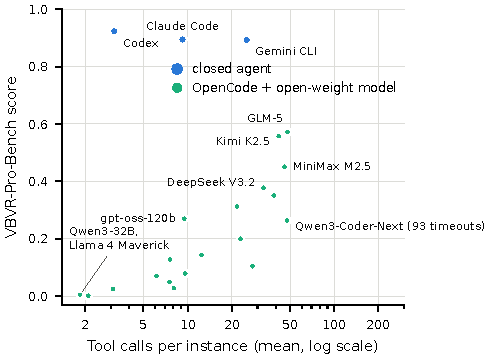
\includegraphics[width=\linewidth]{figures/fig_tools_vs_score.pdf}
\caption{Score against mean tool calls per instance (log scale) for every lane that produced at least one video, the disc area proportional to the number of videos produced out of 500; the four lanes with no video are omitted. Dark blue discs are the closed agents, light blue OpenCode with an open-weight model; the three closed agents sit at the top left, and no lane to their right reaches them. Values from \cref{tab:efficiency} and its full-length source, \texttt{bench/paper/table3\_efficiency.csv}.}
\label{fig:tools}\vspace{-8pt}
\end{wrapfigure}
The three closed agents land within 0.030 of each other, but they do not pay the same price (\cref{tab:efficiency}). Codex solves an instance in 3.2 tool calls, a median of 22\,s and 56.8k input tokens. Claude Code uses 2.9$\times$ the calls, 4.8$\times$ the time and 4.1$\times$ the input tokens for a score 0.029 lower; Gemini CLI uses 8.0$\times$ the calls, 9.9$\times$ the time and 11.6$\times$ the input tokens for a score 0.030 lower. The difference lies in how each agent looks at the frame. Codex receives the frame as an image attached to its prompt, and a typical trace is a directory listing, one probe of a few pixels and the program, three commands in all. Claude Code opens the image with its file reader on 465 of the 500 instances, then measures coordinates with short scripts. Gemini CLI opens the image on only 10 of 500 instances. It reconstructs the scene numerically, script by script, and the 25.3 calls and 659k input tokens per instance are the cost of that reconstruction.

\Cref{fig:tools} puts every lane on one axis. Calls do not buy score. The best open-weight lanes, GLM-5 and Kimi K2.5, make 48.0 and 41.9 calls per instance and read 1.57M and 1.21M input tokens, 15$\times$ and 13$\times$ Codex's calls and 28$\times$ and 21$\times$ its tokens, for 0.572 and 0.557. The lanes that call tools the least also score the least, so tool use is necessary, and yet it fails to separate the top three from the rest.

% Generated from bench/paper/table3_efficiency.csv (agents' own event logs; 500 instances per lane).
\begin{table*}[t]
\centering
\caption{Cost of a solution. Per-instance means over the 500 instances (median for wall-clock seconds), from each agent's own event log. Tool-use rate is the fraction of instances with at least one tool call; tokens are input/output per instance in thousands; timeouts are instances killed at the 1800\,s wall clock. The three closed agents and the six best open-weight lanes are shown; every lane that produced a video appears in \cref{fig:tools}.}
\label{tab:efficiency}
\small
\setlength{\tabcolsep}{5pt}
\begin{tabular}{lrrrrrrrr}
\toprule
Agent & Score & Videos & Tool use & Calls & Median s & In (k) & Out (k) & Timeouts \\
\midrule
\textbf{Codex (gpt-6-astra)} & \textbf{0.923} & \textbf{500} & \textbf{1.00} & \textbf{3.2} & \textbf{22} & \textbf{57} & \textbf{1.2} & \textbf{0} \\
Claude Code (Fable 5.1) & 0.894 & 500 & 1.00 & 9.2 & 105 & 233 & 7.3 & 0 \\
Gemini CLI (Gemini 3.1 Pro) & 0.893 & 500 & 1.00 & 25.3 & 218 & 659 & 7.5 & 0 \\
\midrule
GLM-5 & 0.572 & 495 & 1.00 & 48.0 & 378 & 1569 & 16.3 & 12 \\
Kimi K2.5 & 0.557 & 498 & 0.99 & 41.9 & 336 & 1213 & 19.2 & 0 \\
MiniMax M2.5 & 0.451 & 488 & 0.99 & 45.7 & 420 & 1295 & 19.8 & 0 \\
DeepSeek V3.2 & 0.378 & 475 & 1.00 & 32.9 & 277 & 636 & 13.6 & 0 \\
Devstral 2 123B & 0.350 & 494 & 0.99 & 38.7 & 344 & 839 & 13.1 & 0 \\
Kimi K2 Thinking & 0.313 & 406 & 0.96 & 21.8 & 125 & 509 & 15.5 & 1 \\
\bottomrule
\end{tabular}
\end{table*}


\subsection{Failure Anatomy of the Open-Weight Lanes}
\label{sec:ana-failure}

An instance fails in one of two ways: a \emph{delivery failure}, in which no \texttt{video.mp4} exists when the container exits, or a \emph{content failure}, in which a video exists and the evaluator rejects it. \Cref{tab:efficiency} separates the two through the \emph{Videos} column, and the source CSV further splits delivery failures by whether the agent called a tool at all.

\textbf{No tool call.} Gemma 3 27B, Gemma 3 12B, Llama 3.3 70B and Magistral Small never call a tool on any of their 500 instances. They answer the instruction in prose. Gemma 3 27B on G-13 writes ``Okay, I will write a Python script to generate the video as described in the prompt'' and then prints a script whose coordinates are \texttt{green\_start = (100, 100)} with the comment ``This is a placeholder, and you'll need to implement logic to detect these colors'' (lane \texttt{bedrock-gemma-3-27b}, G-13, instance 00000). Llama 3.3 70B emits the tool call itself as text, \texttt{\{"type": "function", "name": "write", "parameters": ...\}}, with \texttt{waypoints = [(100, 100), (200, 200), (300, 300)]  \# Replace with actual waypoints} inside it (lane \texttt{bedrock-llama3.3-70b}, G-13, instance 00000); the call is never executed. All four score 0 for the same reason a video model that fails to generate scores 0.

\textbf{One or two calls, then stop.} Qwen3-32B averages 1.85 calls per instance and delivers 25 videos; Llama 4 Maverick averages 2.10 calls and delivers 7. Qwen3-32B reads a file or writes a skeleton and hands the work back: ``The skeleton code for the video generator has been created at \texttt{/app/solve.py}. Next, you need to implement the logic for finding the green and red positions'' (lane \texttt{bedrock-qwen3-32b}, G-13, instance 00000). Llama 4 Maverick delegates to a sub-agent type that does not exist, fetches a web page, and stops. 475 and 482 of their instances are delivery failures with a tool call on record.

\textbf{Timeouts.} Qwen3-Coder-Next is the opposite failure. It calls 47.7 tools per instance, reads 1.82M input tokens, delivers a video on 498 instances, and hits the 1800\,s wall clock on 93 of them, more than every other lane combined; its score is 0.264.

\textbf{Diligent but wrong.} GLM-5, Kimi K2.5 and MiniMax M2.5 make 42--48 calls per instance, read 1.2--1.6M input tokens, and deliver a video on 495, 498 and 488 instances. Their failures are almost all content failures: their scores over delivered videos, 0.578, 0.560 and 0.462, are within 0.011 of their scores over all 500. These models run the loop the closed agents run, at a higher price, and produce a wrong video.

\subsection{Where the Closed Agents Fail}
\label{sec:where-fail}

On 53 of the 100 tasks all three agents score at least 0.95, and on 13 the three-agent mean is below 0.7 (\cref{fig:heatmap}). \Cref{tab:hardest} lists the twelve hardest; eleven are in-domain. We read the programs and the evaluators behind these tasks and find four causes\IfFileExists{figures/fig_qualitative.pdf}{; \cref{fig:qualitative} shows the agents' last frames beside the ground truth on ten tasks, three of them from \cref{tab:hardest}}{}.

\begin{figure}[!htb]
\centering
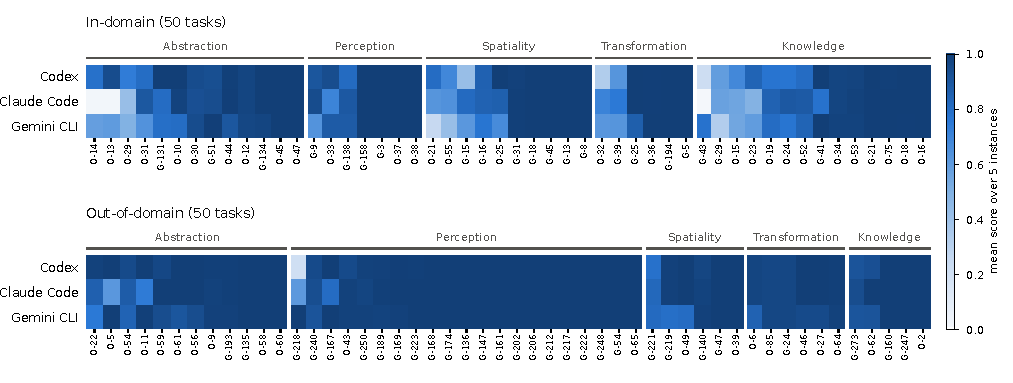
\includegraphics[width=\textwidth]{figures/fig_heatmap.pdf}
\caption{Per-task mean score of the three closed agents on all 100 tasks, the 50 in-domain tasks in the left block and the 50 out-of-domain tasks in the right, grouped by category (labels above). Colour is one ramp from 0 (white) to 1 (dark blue); the 13 tasks with a three-agent mean below 0.7 are named under the axis, and the twelve of \cref{tab:hardest} are among them. Values from \texttt{bench/paper/table4\_per\_task\_closed.csv}; categories from the evaluator output.}
\label{fig:heatmap}
\end{figure}

% Generated from bench/paper/table4_per_task_closed.csv (per-task mean over 5 instances; category from the evaluator results).
\begin{table*}[t]
\centering
\caption{The twelve hardest tasks for the closed agents: lowest mean of the three per-task scores (each a mean over 5 instances). Split is in-domain (ID) or out-of-domain (OOD); category is the benchmark's. \cref{sec:where-fail} groups them by cause.}
\label{tab:hardest}
\small
\setlength{\tabcolsep}{5pt}
\begin{tabular}{llllrrrr}
\toprule
Task & Name & Split & Category & Codex & Claude & Gemini & Mean \\
\midrule
G-43 & understand scene structure & ID & Knowledge & 0.21 & 0.00 & \textbf{0.77} & 0.33 \\
O-14 & shape scale then outline & ID & Abstraction & \textbf{0.78} & 0.01 & 0.58 & 0.45 \\
G-29 & chart extreme with data & ID & Knowledge & \textbf{0.59} & 0.57 & 0.32 & 0.49 \\
O-13 & shape outline then move & ID & Abstraction & \textbf{0.94} & 0.01 & 0.59 & 0.51 \\
O-29 & ballcolor & ID & Abstraction & \textbf{0.73} & 0.41 & 0.49 & 0.54 \\
O-32 & rolling ball & ID & Transformation & 0.32 & \textbf{0.70} & 0.61 & 0.54 \\
O-21 & construction blueprint & ID & Spatiality & \textbf{0.80} & 0.62 & 0.24 & 0.55 \\
O-55 & rotation & ID & Spatiality & \textbf{0.68} & 0.64 & 0.41 & 0.58 \\
O-15 & ball bounces given time & ID & Knowledge & \textbf{0.68} & 0.55 & 0.54 & 0.59 \\
G-218 & identify largest angle in triangle & OOD & Perception & 0.20 & 0.60 & \textbf{1.00} & 0.60 \\
G-15 & grid avoid obstacles & ID & Spatiality & 0.41 & \textbf{0.81} & 0.61 & 0.61 \\
O-23 & domino chain branch path prediction & ID & Knowledge & \textbf{0.83} & 0.48 & 0.59 & 0.63 \\
\bottomrule
\end{tabular}
\end{table*}


\textbf{The answer belongs where the diagram puts it.} O-13 and O-14 show an analogy $A\!\to\!B\!\to\!C :: D\!\to\,?\!\to\,?$ and ask to ``apply the same two-step transformation''. The two \texttt{?} cells are where the answer belongs, and the top row's ``filled'' and ``outline'' styles differ only in stroke width. Claude Code animates $D$ in place on all 10 instances of the two tasks, thinning its stroke and moving it, and scores below 0.1 on every one; Gemini CLI does so on 4 of 10. Codex writes into the \texttt{?} cells on all 10 and scores 0.9 or above on 9; on the tenth it redraws the shape instead of copying its pixels and scores 0.

\textbf{Unstated conventions decide the score.} On G-218 every program we read detects the three vertices and computes the largest interior angle in the same way; the scores follow the radius of the drawn circle, not the vertex. The evaluator credits a circle only if it covers 70\% of an $80\times80$ pixel box around the vertex, and the ground-truth ring has radius 40. Programs that drew a radius of 34 or less score 0 (four of Codex's five instances, two of Claude's); those that drew 37 or more score 1.0 (all five of Gemini's). On G-43 the three agents box the same room on four of the five instances, with boxes that differ by at most 20 pixels, and score 0.00, 0.00 and 0.78 on instance 00000. The evaluator's green range, $R\!\le\!100$, $G\!\ge\!100$, $B\!\le\!100$, contains the floorplan's grey $(100,100,100)$ outlines exactly at its corner. How many of them survive video encoding sets the count of ``green'' contours, and the count penalty removes the whole score.

\textbf{A correct answer that is not the reference.} G-15 asks for a shortest path around obstacles. Any shortest path is correct, but the evaluator scores proximity to the ground truth's own path. The three programs for instance 00001 each run a breadth-first search; Claude Code's tie-break reproduces the reference path and scores 1.0, Codex's and Gemini's return other paths of the same length and score 0.03 each. On instance 00002, where the shortest path is a straight line, all three score at least 0.999.

\textbf{The frame under-determines the video.} O-55 rotates the camera $180^\circ$ around a six-block sculpture, which reveals faces that are not visible in the frame. O-32 and O-15 are scored against a simulated trajectory whose speed and timing the prompt does not give. O-29, O-21 and O-23 grade a multi-step process on the order and state of its intermediate steps. G-29 requires reading numeric labels off a pie chart, and scores swing from 0.0 to 0.96 between instances. On these tasks a program alone is not enough, and a physical or perceptual prior would help. Eleven of the twelve hardest tasks are in-domain, and this is the source of the agents' higher score on the held-out half.

\IfFileExists{figures/fig_qualitative.pdf}{%
\begin{figure}[H]
\centering
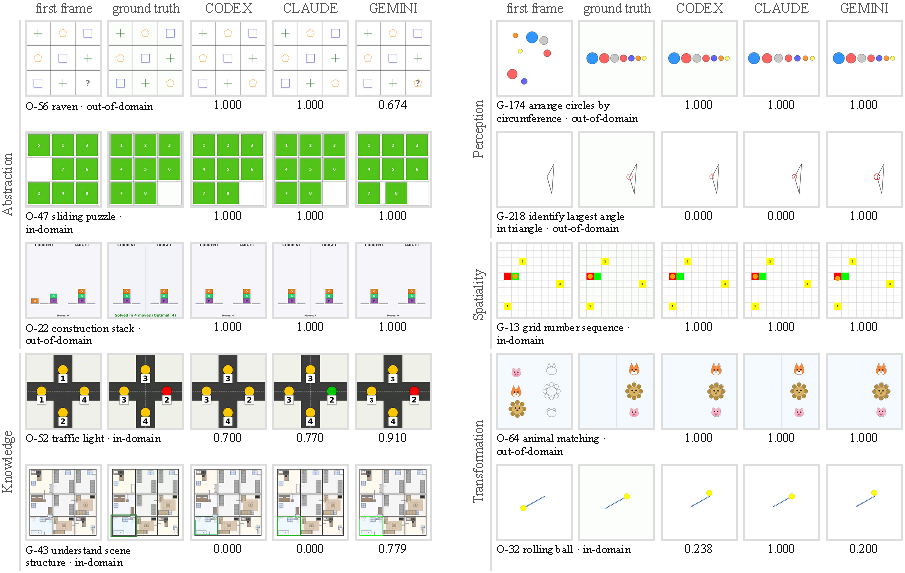
\includegraphics[width=\textwidth]{figures/fig_qualitative.pdf}
\caption{Last frames of the three closed agents beside the ground truth on ten tasks (instance 00000), grouped by category. Each row shows the first frame the agent was given, the ground-truth last frame and the last frame rendered by the program Codex, Claude Code and Gemini CLI wrote, with the official evaluator's score under each. Most rows are solved by all three; the failures are the unstated conventions of G-43 and G-218 (\cref{sec:where-fail}), where the drawn box or circle sits in the right place and scores 0, and the under-determined trajectory of O-32, with partial credit on O-52 and O-56.}
\label{fig:qualitative}
\end{figure}
}{}

\subsection{What a Winning Program Does}
\label{sec:ana-qualitative}

\Cref{lst:raven} shows the O-56 program, a $3\times3$ progressive matrix with an empty bottom-right cell. Codex never inspected a pixel. It read the frame attached to its prompt, stated the rule (``each row shifts the three symbols one position left''), and wrote the program in its second command. The program copies the pentagon's own pixels from the cell where it appears into the empty cell, so stroke and colour match the source exactly; it fades the question mark to white over eight frames and reveals the copied pixels in angular order over the next 25; and it asserts, on every frame, that the other eight cells are byte-identical to the input. Its 835 output tokens cover the whole run.

\IfFileExists{figures/fig_code_O56.pdf}{%
\begin{figure}[!htb]
\centering
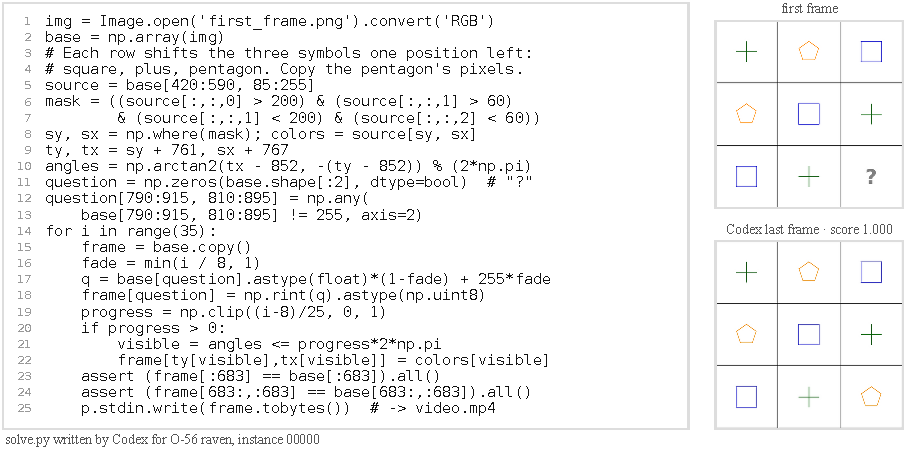
\includegraphics[width=\textwidth]{figures/fig_code_O56.pdf}
\caption{The Codex program for O-56 (raven, out-of-domain, instance 00000; 2 tool calls, 17\,s, score 1.0) beside the task's first frame and the last frame it renders. The program is the agent's own \texttt{solve.py}, trimmed to the lines discussed in the text; it copies the pentagon's pixels from the cell where they appear into the empty cell and asserts on every frame that the other eight cells are unchanged.}
\label{lst:raven}
\end{figure}
}{%
\begin{figure}[H]
\centering
\fontsize{5.8}{6.6}\selectfont
\begin{minipage}[t]{0.49\textwidth}
\verbatiminput{figures/qualitative/O-56_raven.py}
\end{minipage}\hfill
\begin{minipage}[t]{0.49\textwidth}
\verbatiminput{figures/qualitative/G-13_grid_number_sequence.py}
\end{minipage}
\normalsize
\caption{Two Codex programs that score 1.0, trimmed to 25 lines each (imports and the ffmpeg encoder setup removed, long lines wrapped); the trimmed programs reproduce the original frames exactly. Left: O-56 raven, out-of-domain, instance 00000, 2 tool calls, 17\,s. Right: G-13 grid number sequence, in-domain, instance 00000, 3 tool calls, 20\,s.}
\label{lst:raven}\label{lst:grid}
\end{figure}
}

\Cref{lst:grid} shows the G-13 program, which must guide the agent through numbered cells to the goal along shortest grid paths. Codex probed the frame once to find the sprite's bounding box, hard-coded the nine corner cells of the route from its reading of the image, with a comment giving the Manhattan length of each leg, and expanded the corners into a cell-by-cell route. Every frame is the input with the sprite erased from the start cell and re-stamped, pixel for pixel, at an interpolated position, so the board never changes.

\IfFileExists{figures/fig_code_G13.pdf}{\IfFileExists{figures/fig_code_O56.pdf}{%
\begin{figure}[!htb]
\centering
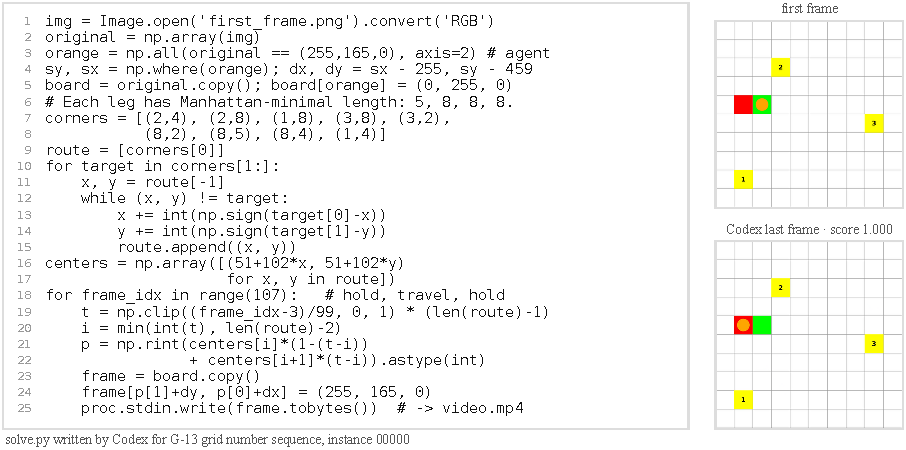
\includegraphics[width=\textwidth]{figures/fig_code_G13.pdf}
\caption{The Codex program for G-13 (grid number sequence, in-domain, instance 00000; 3 tool calls, 20\,s, score 1.0) beside the task's first frame and the last frame it renders. The nine corner cells of the route are written down from the image, each leg annotated with its Manhattan length, and the sprite is erased and re-stamped pixel for pixel on every frame.}
\label{lst:grid}
\end{figure}
}{}}{}

\subsection{Scope of the Result}
\label{sec:ana-scope}

The comparison is exact because both families are graded by the same deterministic evaluator on the same 500 instances, and it is narrow for the same reason. The agents were told the container geometry, had one attempt, and were judged by rules with the sensitivities of \cref{sec:where-fail}; no human looked at a video. The result concerns the interface, a program against a denoiser, on a benchmark built to be verifiable. It does not show that the agents perceive the frame better than a video model in general.
